% Options for packages loaded elsewhere
\PassOptionsToPackage{unicode}{hyperref}
\PassOptionsToPackage{hyphens}{url}
%
\documentclass[final,11pt]{article}

% Essential packages
\usepackage[T1]{fontenc}
\usepackage[utf8]{inputenc}
\usepackage[margin=1in]{geometry}
\usepackage{amsmath,amssymb,amsthm}
\usepackage{graphicx}
\usepackage{url}
\usepackage{hyperref}

% Hyperref setup
\hypersetup{
  pdftitle={Time Series Analysis - STAT 478 - Project},
  pdfauthor={Alexander Towell (atowell@siue.edu)},
  pdfkeywords={time series analysis, known-plaintext attack, encrypted search, confidentiality measure, estimation},
  hidelinks,
  pdfcreator={LaTeX}}

% Custom commands (from alex.sty)
\newcommand{\backshift}{\operatorname{B}}
\newcommand{\arima}{\operatorname{ARIMA}}
\newcommand{\argmax}{\operatorname{arg\,max}}
\newcommand{\set}[1]{\mathbb{#1}}

% Indicator function - use simple 1 instead of mathbbm
\newcommand{\indicator}[1]{\mathbf{1}_{#1}}

% Theorem environments
\theoremstyle{plain}
\newtheorem{theorem}{Theorem}
\newtheorem{definition}{Definition}
\newtheorem{assumption}{Assumption}

\theoremstyle{remark}
\newtheorem*{remark}{Remark}

% Figure settings
\makeatletter
\def\maxwidth{\ifdim\Gin@nat@width>\linewidth\linewidth\else\Gin@nat@width\fi}
\def\maxheight{\ifdim\Gin@nat@height>\textheight\textheight\else\Gin@nat@height\fi}
\setkeys{Gin}{width=\maxwidth,height=\maxheight,keepaspectratio}
\def\fps@figure{htbp}
\makeatother

% Spacing
\setlength{\parindent}{0pt}
\setlength{\parskip}{6pt plus 2pt minus 1pt}
\setlength{\emergencystretch}{3em}
\setcounter{secnumdepth}{5}

\title{Time Series Analysis of Confidentiality Degradation in Encrypted Search Systems}
\author{Alexander Towell \thanks{\href{mailto:atowell@siue.edu}{\nolinkurl{atowell@siue.edu}}} \\ Southern Illinois University-Edwardsville Math Department}
\date{April 30, 2021}

\begin{document}
\maketitle
\begin{abstract}
We present a time series analysis of confidentiality degradation in
encrypted search systems subject to known-plaintext attacks. By modeling
the adversary's accuracy as a time-dependent confidentiality measure, we
develop forecasting models based on ARIMA and dynamic regression techniques.
Our analysis provides quantitative estimates for how quickly adversary
knowledge accumulates, enabling organizations to establish data-driven
policies for password rotation and system reinitialization that maintain
specified confidentiality thresholds.
\end{abstract}

{
\setcounter{tocdepth}{3}
\tableofcontents
}
\hypertarget{introduction}{%
\section{Introduction}\label{introduction}}

Cloud computing enables organizations to store and process data on remote
infrastructure, but this convenience comes at the cost of reduced control
over data confidentiality. Even when data is encrypted at rest, system
administrators and other insiders pose a significant threat. This tension
between utility and security has motivated the development of encrypted
search systems.

Encrypted search attempts to resolve the fundamental trade-off between
confidentiality and usability by enabling authorized users to query
encrypted data without revealing query contents to untrusted parties.

\begin{definition}
Encrypted search allows authorized search agents to investigate the presence
of specific search terms in a confidential target data set, such as a database
of encrypted documents, while the contents---especially the meaning of the target
data set and search terms---are hidden from unauthorized personnel, including
the system administrators of a cloud server.
\end{definition}

Essentially, encrypted search enables oblivious queries where users can
search confidential databases on untrusted systems without revealing their
information needs (and in more sophisticated systems, without revealing which
documents matched the query).

We define the \emph{adversary} as any untrusted party with access to the
remote system where confidential data is stored.\footnote{System administrators
are typical examples.}

However, perfect confidentiality is not achievable in practice. Encrypted
search systems leak information through access patterns, query frequencies,
and other side channels. In this paper, we focus on an adversary who attempts
to infer the plaintext queries by analyzing the history of encrypted searches
using a known-plaintext attack.

We quantify confidentiality using the proportion of queries the adversary
successfully decodes. Since confidentiality degrades as the adversary observes
more queries, we model this degradation as a time series process.

Time series analysis enables us to forecast future confidentiality levels,
answering critical security questions such as: How long until confidentiality
falls below an acceptable threshold? When should passwords be reset to
maintain a minimum confidentiality level?

These forecasts support data-driven security policies. Password resets impose
usability and security costs, but delaying them risks unacceptable
confidentiality loss. Our analysis provides quantitative guidance for
balancing these competing concerns.

\hypertarget{encrypted-search-model}{%
\section{Encrypted search model}\label{encrypted-search-model}}

\label{sec:es_model} In information retrieval, a \emph{search agent}
submits a \emph{query} representing an \emph{information need} to an
information system, which responds with relevant objects (e.g., documents).

We make the following simplifying assumptions about the query model and
encryption scheme.

\begin{assumption}
Queries consist of sequences of keywords (a bag-of-words model).
\end{assumption}

\begin{assumption}
The encrypted search system uses a deterministic encryption scheme where
each plaintext keyword maps to a unique encrypted token (trapdoor).
\end{assumption}

More formally, we define the encryption function as
\begin{equation}
    \operatorname{h} \colon \set{X} \mapsto \set{Y}\,,
\end{equation}
where $\set{X}$ is the set of plaintext search keywords and $\set{Y}$ is
the set of encrypted tokens (trapdoors).

\begin{definition}[Trapdoor]
A trapdoor is a cryptographic token generated by applying $\operatorname{h}$
to a plaintext keyword, enabling the untrusted system to perform searches
without learning the plaintext.
\end{definition}

Since $\operatorname{h}$ is injective, there exists an inverse function
\begin{equation}
    \operatorname{g} \colon \set{Y} \mapsto \set{X}
\end{equation}
such that $x = \operatorname{g}(\operatorname{h}(x))$ for every $x \in \set{X}$.

\begin{definition}
The adversary can observe the sequence of encrypted queries (trapdoors)
submitted by authorized search agents but does not initially know
$\operatorname{g}$.
\end{definition}

The security objective is to prevent the adversary from learning
$\operatorname{g}$ and thus decoding the queries.

We now formalize the time series notation. Following standard conventions,
we use uppercase letters for random variables and lowercase for realizations.
A time series $\{Y_t\}$ denotes a sequence of random variables indexed by
time $t$, with $\{y_t\}$ denoting an observed realization.

The plaintext queries form a discrete-time, discrete-valued time series
$\{x_t\}$ where $x_t \in \set{X}$ is the $t$-th keyword submitted by search
agents. The adversary cannot observe $\{x_t\}$ directly.

\begin{definition}
The encrypted query sequence $\{c_t\}$ is defined by
$$
  c_t = \operatorname{h}(x_t)\,,
$$
where $c_t \in \set{Y}$ is the trapdoor corresponding to plaintext $x_t$.
\end{definition}

We model queries probabilistically as a random process $\{X_t\}$ with
distribution determined by a language model:
\begin{equation}
    \Pr(X_t = x_t | X_{t-1} = x_{t-1},\ldots,X_1 = x_1).
\end{equation}
This formulation assumes queries depend only on query history, not on
external factors such as user identity or time of day. We discuss
extensions to include such covariates in Section~\ref{sec:future}.

The encrypted query sequence is then modeled as the random process
$\{C_t\}$ where $C_t = \operatorname{h}(X_t)$.

\hypertarget{threat-model-known-plaintext-attack}{%
\section{Threat model: known-plaintext
attack}\label{threat-model-known-plaintext-attack}}

\label{sec:threat} The adversary observes the encrypted query sequence
$\{c_t\}$ and attempts to recover the plaintext sequence $\{x_t\}$ by
learning the decryption function $\operatorname{g}$. We focus on
frequency-based cryptanalysis, specifically known-plaintext attacks.
Side-channel information is not considered in this work; we discuss
potential extensions in Section~\ref{sec:future}.

\begin{assumption}
The decryption function $\operatorname{g}$ is unknown to the adversary.
\end{assumption}

The adversary's strategy is to estimate $\operatorname{g}$ by exploiting
statistical properties of natural language. Given observed ciphers
$\{c_1,\ldots,c_T\}$, a maximum likelihood estimator of $\operatorname{g}$
is
\begin{equation}
\label{eq:mle}
    \hat{\operatorname{g}} = \argmax_{\operatorname{g} \in G}
    \Pr(X_1 = \operatorname{g}(c_1)) \prod_{t=2}^{T} \Pr(X_t =
    \operatorname{g}(c_t) | X_{t-1} = \operatorname{g}(c_{t-1}),
            \ldots, X_1 = \operatorname{g}(c_1))\,,
\end{equation}
where $G$ denotes the set of all injective functions from $\set{Y}$ to
$\set{X}$.

Perfect confidentiality would require that all plaintexts be equally likely,
making them indistinguishable to the adversary. In this case,
$\hat{\operatorname{g}}$ would be inconsistent. However, natural language
exhibits strong statistical regularities (word frequencies follow Zipf's law,
co-occurrence patterns are non-uniform), enabling the adversary to learn
something about $\{x_t\}$ from $\{c_t\}$.

In practice, the adversary does not know the true distribution of $\{X_t\}$
but can approximate it using external corpora.

\begin{assumption}
The adversary has access to an approximate language model
$\hat{\Pr}(\cdot)$ for the query distribution.
\end{assumption}

\begin{definition}
In a \emph{known-plaintext attack}, the adversary estimates
$\operatorname{g}$ by solving the MLE in Equation~\eqref{eq:mle} with
the true distribution replaced by the approximate distribution
$\hat{\Pr}(\cdot)$.
\end{definition}

The quality of the attack depends on how well $\hat{\Pr}(\cdot)$ approximates
the true query distribution.

\section{Confidentiality measure}

We quantify confidentiality degradation using the adversary's decryption
accuracy.

\begin{definition}
The confidentiality measure $\{\pi_t\}$ is defined as the fraction of
ciphers correctly decoded by the adversary using $\hat{\operatorname{g}}$:
\begin{equation}
\label{eq:accuracy}
    \pi_t = \frac{\delta_t}{Nt}\,,
\end{equation}
where
\begin{equation}
    \delta_t = \sum_{t'=1}^{Nt} \mathbf{1}[\operatorname{g}(c_{t'}) = \hat{\operatorname{g}}(c_{t'})]\,.
\end{equation}
Here $N$ is a sampling parameter: we compute one measurement of $\pi_t$
after every $N$ queries.
\end{definition}

The measure $\pi_t$ represents the proportion of the entire query history
that the adversary can decode at time $t$. Note that $\pi_t$ increases as
the adversary observes more queries and refines $\hat{\operatorname{g}}$.

\subsection{Security threshold and password rotation}

Suppose we require that confidentiality remain above a threshold $\pi^* \in (0,1)$.
We define the critical time $T^*$ as
\begin{equation}
  T^* = \min\{T : \pi_T > \pi^*\}\,.
\end{equation}
At time $T^*$, the adversary can decode more than proportion $\pi^*$ of
queries, violating the security requirement.

To maintain the threshold, we must reinitialize the encryption before
reaching $T^*$. This typically involves changing the cryptographic key
(e.g., requiring password changes), which generates a new encryption
function $\operatorname{h}'$ and resets the adversary's knowledge.
The adversary must then restart the attack process with
$\hat{\operatorname{g}}'$.

Forecasting $\{\pi_t\}$ enables proactive security policies: we can
predict when $\pi_t$ will exceed $\pi^*$ and schedule reinitialization
accordingly.

\hypertarget{forecasting-model}{%
\subsection{Forecasting model}\label{forecasting-model}}

Since $\{c_t\}$ is random, the confidentiality measure $\{\pi_t\}$ is
also random. We model it as a stochastic process $\{\Pi_t\}$.

Given observations $\pi_1,\ldots,\pi_T$, the $h$-step ahead forecast
distribution is
$$
\Pi_{T+h|T} \equiv (\Pi_{T+h} \mid \Pi_1 = \pi_1,\ldots,\Pi_T = \pi_T)\,.
$$
The forecast mean is denoted $\mathbb{E}[\Pi_{T+h|T}]$.

Our goal is to estimate the forecast distribution from observed data. In
practice, we estimate the forecast mean $\hat{\pi}_{T+h|T}$ and construct
prediction intervals using the estimated forecast variance.

\hypertarget{data-description}{%
\section{Data description}\label{data-description}}

We analyze simulated data to evaluate forecasting models for $\{\pi_t\}$.
The simulation generates realistic query sequences and models an adversary
conducting a known-plaintext attack.

\subsection{Data generation}

The simulation proceeds in two phases: query generation and attack simulation.

\paragraph{Query generation.}
We first generate a synthetic plaintext query sequence $\{x_t\}$:
\begin{enumerate}
\item A bigram language model is estimated from a text corpus. (The specific
corpus has been lost; it was a general English text collection.)
\item Plaintext queries $\{x_t\}$ are sampled from this bigram model.
\item Each plaintext $x_t$ is encrypted via a cryptographic hash function
to produce ciphers $c_t = \operatorname{h}(x_t)$.
\end{enumerate}

\paragraph{Attack simulation.}
Given the cipher sequence $\{c_t\}$, we simulate an adversary attempting
to learn $\operatorname{g}$:
\begin{enumerate}
\item After every $N=50$ ciphers, the adversary updates its estimate
$\hat{\operatorname{g}}$ by solving a unigram MLE:
$$
    \hat{\operatorname{g}}_T = \argmax_{\operatorname{g} \in G}
    \prod_{t=1}^{T} \hat{\Pr}(X_t = \operatorname{g}(c_t))\,.
$$
Note that the adversary uses a unigram model even though queries were
generated from a bigram model. This reflects information loss in practice.
\item The adversary's language model $\hat{\Pr}(\cdot)$ is estimated from
a different corpus than the one used to generate $\{x_t\}$. This mismatch
makes $\hat{\operatorname{g}}_T$ inconsistent (it does not converge to
$\operatorname{g}$ as $T \to \infty$), reflecting realistic conditions
where the adversary's knowledge is imperfect.
\item The confidentiality measure $\pi_t$ is computed using the current
estimate $\hat{\operatorname{g}}_t$.
\end{enumerate}

This setup models a realistic scenario where the adversary has approximate
but not perfect knowledge of the query distribution.

\hypertarget{time-series-analysis-of-pi_t}{%
\section{\texorpdfstring{Time series analysis of
\(\{\pi_t\}\)}{Time series analysis of \textbackslash\{\textbackslash pi\_t\textbackslash\}}}\label{time-series-analysis-of-pi_t}}

The adversary's accuracy exhibits temporal dependence: accuracy at time $t$
is correlated with recent values $\pi_{t-1}, \pi_{t-2}, \ldots$, with
correlation typically decreasing as lag increases. This autocorrelation
structure motivates time series methods for forecasting.

We partition the data into training and test sets. The training set is used
for model fitting and the test set is held out for evaluation. Sample
training data:

\begin{verbatim}
## [1] 0.358159 0.351208 0.347271 0.346403 0.352666 0.350445
\end{verbatim}

\hypertarget{visualization-and-stationary-transformations}{%
\subsection{Visualization and stationary
transformations}\label{visualization-and-stationary-transformations}}

ARIMA models assume stationarity: constant mean, constant variance, and
autocorrelation that depends only on lag. We must transform $\{\pi_t\}$ to
approximate stationarity before fitting ARIMA models.

Figure~\ref{fig:fa} plots the training data. The series exhibits an
upward trend, indicating non-stationarity in the mean.

\begin{figure}
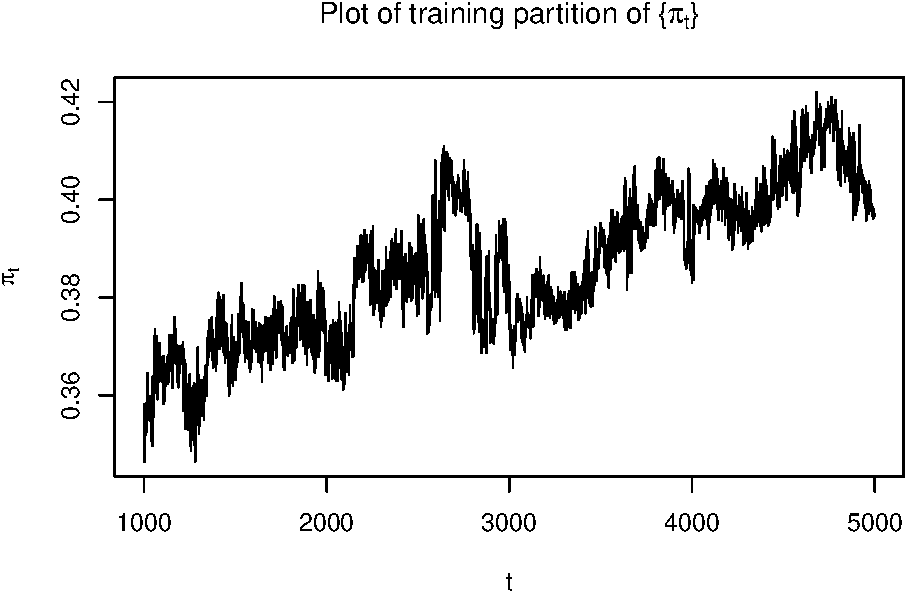
\includegraphics{paper_files/figure-latex/unnamed-chunk-2-1.pdf}
\caption{Time series plot of $\{\pi_t\}$ showing non-stationary behavior.}
\label{fig:fa}
\end{figure}

Figure~\ref{fig:f0} shows the sample ACF and PACF. The slow decay in the
ACF confirms non-stationarity.

\begin{figure}
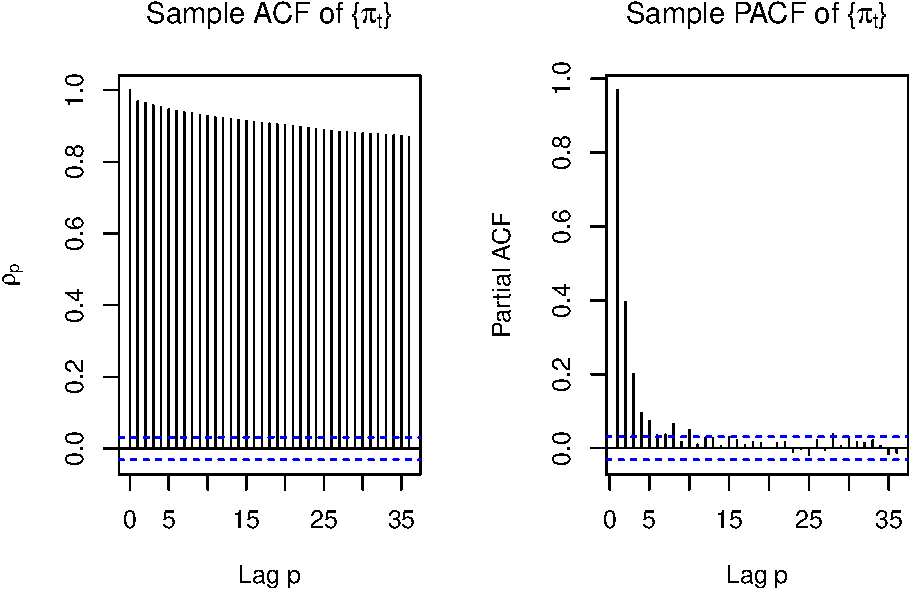
\includegraphics{paper_files/figure-latex/unnamed-chunk-3-1.pdf}
\caption{Sample ACF and PACF showing strong autocorrelation.}
\label{fig:f0}
\end{figure}

The variance appears reasonably constant, so variance-stabilizing
transformations (e.g., logarithm) are unnecessary. To remove the trend,
we apply differencing: the $d$-th order differenced series is denoted
$\nabla^d\{\pi_t\}$. Differencing is a flexible, non-parametric approach
that adapts to complex trend patterns without assuming a specific
functional form.

\begin{figure}
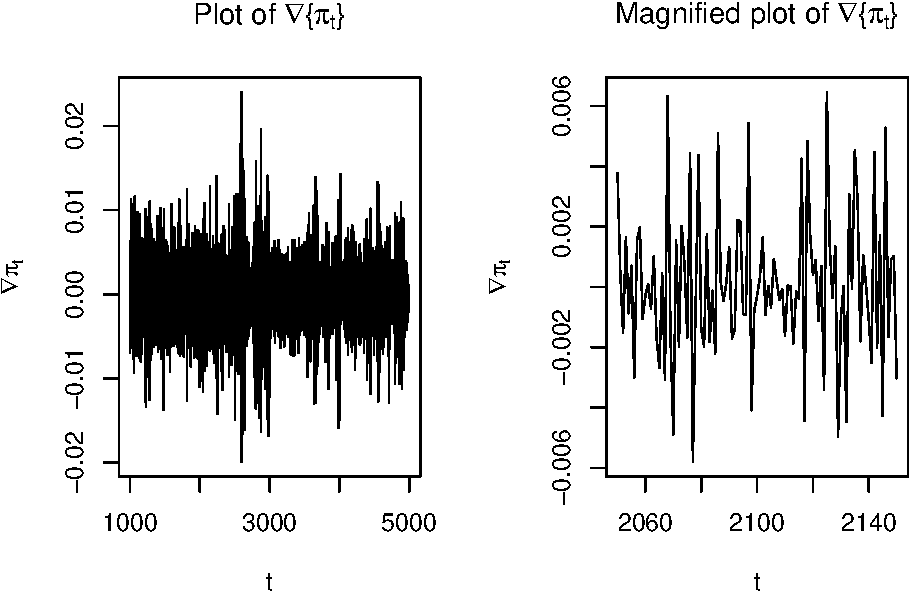
\includegraphics{paper_files/figure-latex/unnamed-chunk-4-1.pdf}
\caption{First-differenced series $\nabla \{\pi_t\}$.}
\label{fig:f1}
\end{figure}

Figure~\ref{fig:f1} shows the differenced series $\nabla\{\pi_t\}$. The
trend is removed, values fluctuate around zero, and variance appears
constant. This suggests stationarity.

We apply the augmented Dickey-Fuller test~\cite{noauthor_dickeyfuller_2021}
to formally test for stationarity:

\begin{verbatim}
## Augmented Dickey-Fuller Test
## Dickey-Fuller = -20.37, Lag order = 15, p-value = 0.01
## alternative hypothesis: stationary
\end{verbatim}

The $p$-value of 0.01 provides strong evidence against the null hypothesis
of non-stationarity. We conclude that $\nabla\{\pi_t\}$ is approximately
stationary and proceed with ARIMA modeling.

\hypertarget{arima-model-selection}{%
\subsection{ARIMA model selection}\label{arima-model-selection}}

Our goal is to build a parsimonious forecasting model. Following Occam's
razor, simpler models with fewer parameters are preferred: they generalize
better to unseen data and avoid overfitting~\cite{bias_variance}. However,
the model must be sufficiently complex to capture the data's structure.
This is the classical bias-variance tradeoff.

ARIMA$(p,d,q)$ models are parameterized by three integers: $p$
(autoregressive order), $d$ (differencing order), and $q$ (moving average
order). We seek small values of $p$, $d$, and $q$ that adequately fit the
data. While information criteria like AIC can guide selection, we also
examine diagnostic plots.

Figure~\ref{fig:f3} shows the ACF and PACF of $\nabla\{\pi_t\}$.

\begin{figure}
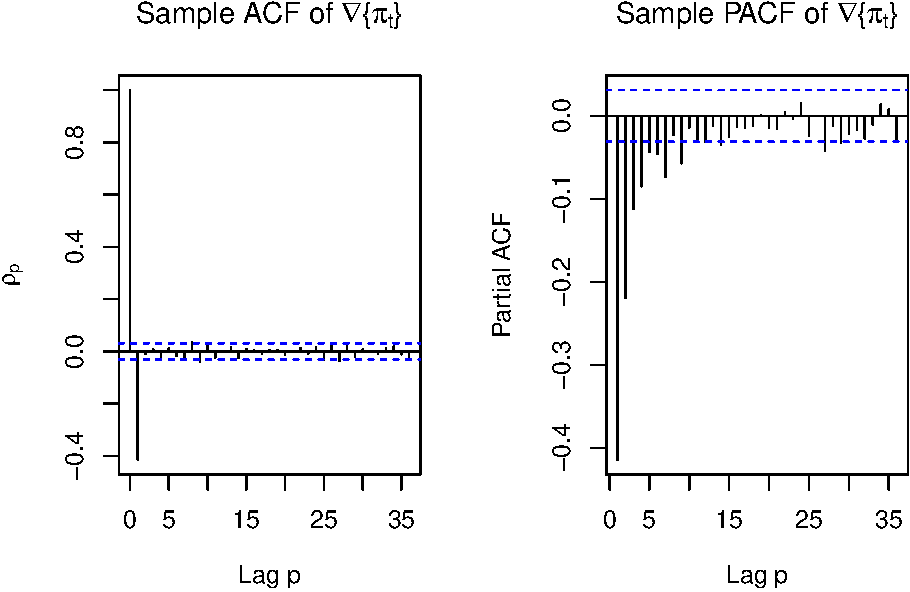
\includegraphics{paper_files/figure-latex/unnamed-chunk-6-1.pdf}
\caption{Sample ACF and PACF of the differenced series $\nabla \{\pi_t\}$.}
\label{fig:f3}
\end{figure}

The ACF cuts off after lag 1, and the PACF decays exponentially,
suggesting an MA(1) process for $\nabla\{\pi_t\}$ (i.e., IMA(1,1) for
$\{\pi_t\}$).

The extended ACF (EACF) table provides additional guidance:

\begin{verbatim}
## AR/MA
##   0 1 2 3 4 5 6 7 8 9 10 11 12 13
## 0 x o o o o o o x x x o  o  o  o
## 1 x x o o o o x o o o o  o  o  o
## 2 x x x o o o x o o o o  o  o  o
## 3 x x x x o o o o o o o  o  o  o
## 4 x x x x x o o o o o o  o  o  o
## 5 x x x x x x o o o o o  o  o  o
## 6 x x x x x o x o o o o  o  o  o
## 7 x x x x x x x o o o o  o  o  o
\end{verbatim}

The EACF suggests candidate models ARMA$(0,1)$, ARMA$(0,2)$, and
ARMA$(1,2)$ for $\nabla\{\pi_t\}$. We evaluate all three.

\hypertarget{model-construction-and-evaluation}{%
\subsection{Model construction and
evaluation}\label{model-construction-and-evaluation}}

Model adequacy is assessed through residual diagnostics. A well-specified
model produces residuals $\{e_t\}$ that behave like white noise:
\begin{enumerate}
\item Uncorrelated: If residuals are correlated, the model has not captured
all temporal structure and can be improved.
\item Zero mean: Non-zero mean residuals indicate systematic bias in forecasts.
\item Constant variance: Heteroscedasticity may require variance modeling.
\end{enumerate}

\hypertarget{ima11}{%
\subsubsection{IMA(1,1)}\label{ima11}}

We first fit ARIMA$(0,1,1)$, the simplest candidate model. The estimated
parameter is:

\begin{verbatim}
##        ma1
## -0.5705635
\end{verbatim}

Figure~\ref{fig:resv} shows residual diagnostics.

\begin{figure}
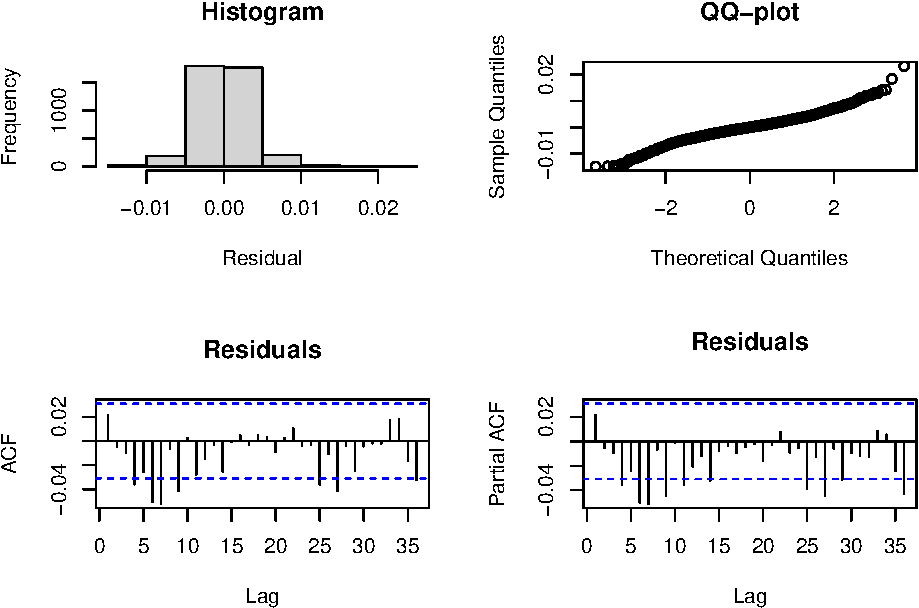
\includegraphics{paper_files/figure-latex/unnamed-chunk-9-1.pdf}
\caption{Residual diagnostics for ARIMA$(0,1,1)$.}
\label{fig:resv}
\end{figure}

The histogram appears symmetric around zero, but the Q-Q plot shows
deviations from normality. More critically, the ACF and PACF exhibit
significant residual autocorrelation, indicating the model has not captured
all temporal dependence. We reject this model.

\hypertarget{ima12}{%
\subsubsection{IMA(1,2)}\label{ima12}}

Next we fit ARIMA$(0,1,2)$. The estimated parameters are:

\begin{verbatim}
##         ma1         ma2
## -0.55254743 -0.04124893
\end{verbatim}

Figure~\ref{fig:res3} shows residual diagnostics.

\begin{figure}
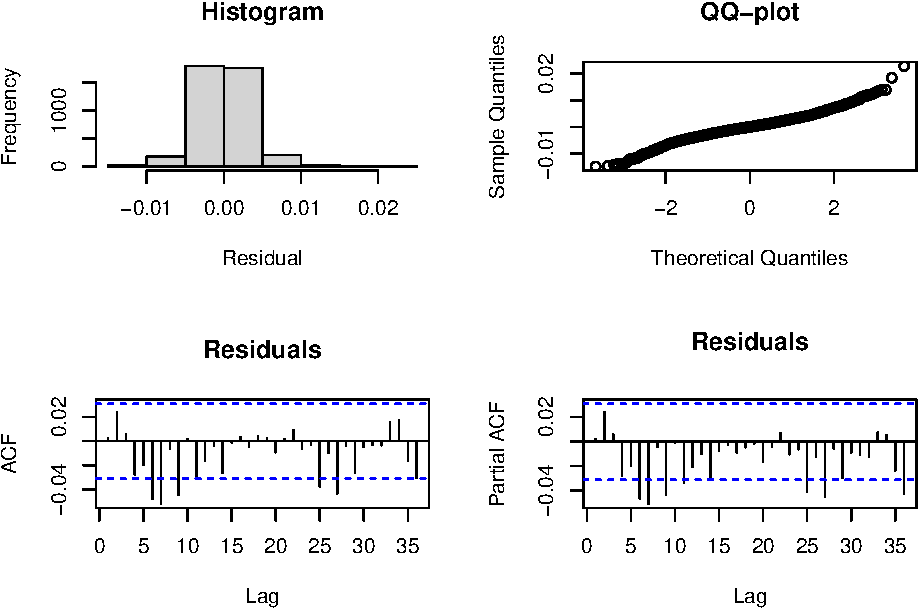
\includegraphics{paper_files/figure-latex/unnamed-chunk-11-1.pdf}
    \caption{Residual diagnostics for ARIMA$(0,1,2)$.}
    \label{fig:res3}
\end{figure}

As before, the histogram is symmetric, and the Q-Q plot indicates
non-normality (though normality is not strictly required for forecasting).
However, the ACF and PACF again show significant residual correlation.
This model is also inadequate. We reject it.

\hypertarget{arima112}{%
\subsubsection{ARIMA(1,1,2)}\label{arima112}}

Finally, we fit ARIMA$(1,1,2)$. The estimated parameters are:

\begin{verbatim}
##        ar1        ma1        ma2
##  0.8839643 -1.4423574  0.4689439
\end{verbatim}

Figure~\ref{fig:res1} shows residual diagnostics.

\begin{figure}
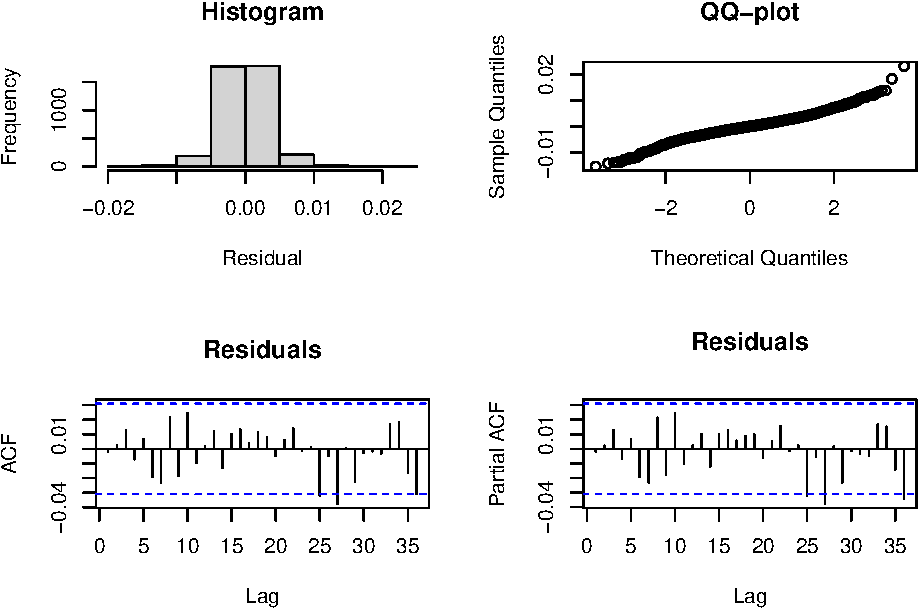
\includegraphics{paper_files/figure-latex/unnamed-chunk-13-1.pdf}
\caption{Residual diagnostics for ARIMA$(1,1,2)$.}
\label{fig:res1}
\end{figure}

Again, the histogram is symmetric and the Q-Q plot shows non-normality.
However, the ACF and PACF appear acceptable: no significant residual
autocorrelation is evident.

We apply the Ljung-Box test (lag 10) to formally assess the white noise
hypothesis:

\begin{verbatim}
## Box-Ljung test
## data: model.3$residuals
## X-squared = 10.333, df = 7, p-value = 0.1705
\end{verbatim}

The null hypothesis is that residuals are white noise. The $p$-value of
0.171 provides substantial support for this hypothesis.

We select ARIMA$(1,1,2)$ as our model. Since this is the only model
passing diagnostics, formal comparison via AIC is unnecessary.

The fitted model summary is:

\begin{verbatim}
## ARIMA(1,1,2)
##
## Coefficients:
##          ar1      ma1     ma2
##       0.8840  -1.4424  0.4689
## s.e.  0.0276   0.0338  0.0266
##
## sigma^2 estimated as 1.088e-05:  log likelihood=17177.64
## AIC=-34347.27   AICc=-34347.26   BIC=-34322.1
\end{verbatim}

In operator form, the model is
\begin{equation}
  (1 - 0.884 \backshift) \nabla \Pi_t = (1 + 1.442 \backshift - 0.469 \backshift^2) e_t\,,
\end{equation}
which factors as
\begin{equation}
  (1 - 0.884 \backshift) \nabla \Pi_t = (1 - 0.273 \backshift) (1 + 1.715 \backshift) e_t\,,
\end{equation}
where $e_t \sim \operatorname{WN}(0, \sigma^2)$ with $\sigma = 0.0033$.

\hypertarget{forecasting}{%
\subsection{Forecasting}\label{forecasting}}

We now use the fitted ARIMA$(1,1,2)$ model to forecast future
confidentiality degradation. At time $T=5000$, we compute forecasts
$\hat{\pi}_{T+h|T}$ for $h = 1, \ldots, 1000$.

Figure~\ref{fig:forecast} shows the forecast along with 80\% prediction
intervals.

\begin{figure}
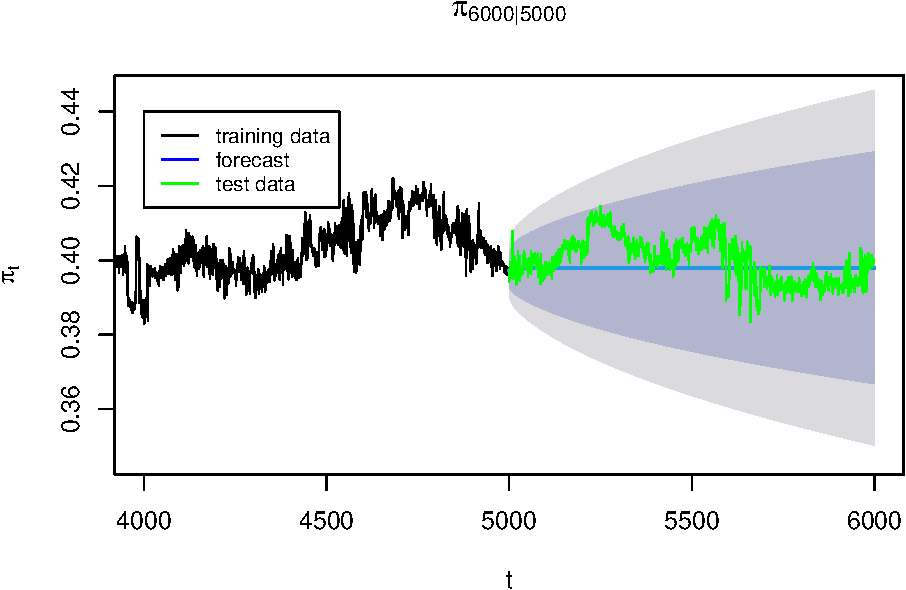
\includegraphics{paper_files/figure-latex/unnamed-chunk-16-1.pdf}
\caption{ARIMA$(1,1,2)$ forecasts with training and test data.}
\label{fig:forecast}
\end{figure}

The held-out test data falls within the 80\% prediction interval for most
time points, suggesting reasonable forecast performance. However, the
prediction intervals are quite wide. We hypothesize this reflects model
misspecification: the purely autoregressive structure may not capture the
underlying process adequately. Theoretically, $\pi_t$ should approach an
asymptotic limit as the adversary's knowledge saturates, but the ARIMA
model does not incorporate this constraint. We explore theory-driven models
in the next section.

\hypertarget{incorporating-information}{%
\subsection{\texorpdfstring{Incorporating \emph{a priori}
information}{Incorporating  information}}\label{incorporating-information}}

We now incorporate domain knowledge about the confidentiality measure.
Assuming the plaintext distribution and encryption function remain fixed,
we expect:

\begin{enumerate}
\item $\pi_t \in [0,1]$ (it is a proportion).
\item $\pi_t$ should be monotonically increasing: observing more queries
cannot decrease the adversary's accumulated knowledge.
\item $\pi_t$ should approach an asymptotic limit $c \leq 1$ as the
adversary's knowledge saturates.
\end{enumerate}

These properties suggest models like Gompertz growth curves or scaled CDFs.
For simplicity, we approximate the trend with a logarithmic function:
\begin{equation}
  \pi_t = \beta_0 + \beta_1 \log t\,.
\end{equation}
While this lacks an asymptote, it provides a reasonable approximation over
finite time horizons.

We model deviations from this trend as ARIMA errors:
\begin{equation}
  \Pi_t = \beta_0 + \beta_1 \log t + \eta_t\,,
\end{equation}
where $\eta_t \sim \arima(p,d,q)$.

Note that this formulation (regression with ARIMA errors) differs from
standard regression. As Hyndman~\cite{rob_arimax} notes, the regression
coefficients condition on lagged responses, complicating interpretation.
Nevertheless, this model can improve forecasts by capturing both the
deterministic trend and stochastic dynamics.

We fit this model to the data:

\begin{verbatim}
## Regression with ARIMA(1,1,2) errors
##
## Coefficients:
##          ar1      ma1     ma2    xreg
##       0.8521  -1.4012  0.4355  0.0292
## s.e.  0.0234   0.0277  0.0211  0.0202
##
## sigma^2 estimated as 6.828e-06:  log likelihood=45279.87
## AIC=-90549.73   AICc=-90549.73   BIC=-90513.68
\end{verbatim}

This uses ARIMA$(1,1,2)$ errors with a logarithmic trend term. (We also
tested ARIMA$(2,1,2)$, which yielded tighter prediction intervals but was
not substantially better.)

Figure~\ref{fig:res} shows residual diagnostics.

\begin{figure}
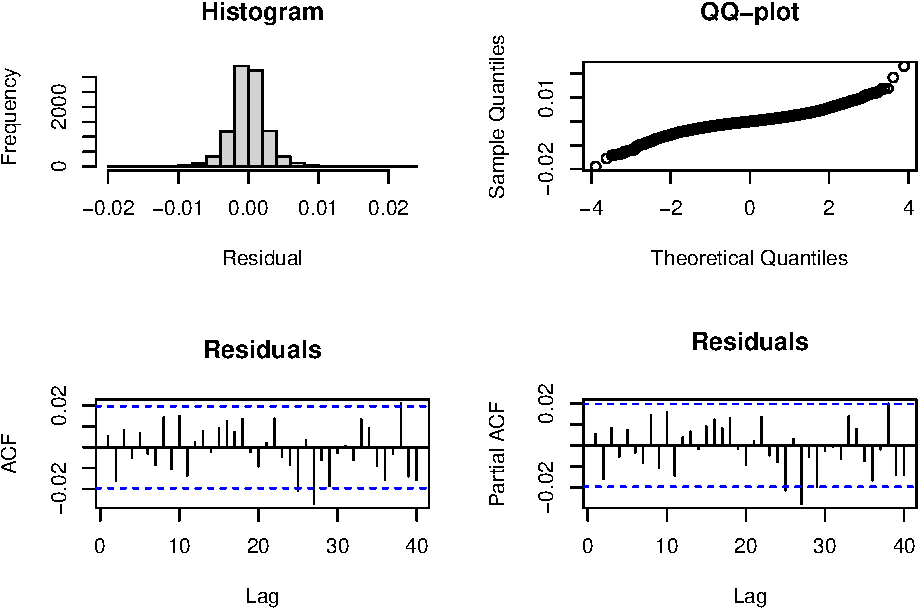
\includegraphics{paper_files/figure-latex/unnamed-chunk-18-1.pdf}
\caption{Residual diagnostics for regression with ARIMA$(1,1,2)$ errors.}
\label{fig:res}
\end{figure}

The histogram is symmetric, the Q-Q plot shows non-normality, and the ACF
and PACF appear acceptable. The Ljung-Box test (lag 10):

\begin{verbatim}
## Box-Ljung test
## data:  reg_model$residuals
## X-squared = 10.279, df = 6, p-value = 0.1134
\end{verbatim}

At the 5\% significance level, the model is marginally adequate
($p = 0.113$). The fitted model is
\begin{equation}
  \hat{\Pi}_t = 0.029 \log t + \eta_t\,,
\end{equation}
where $\eta_t \sim \arima(1,1,2)$ with coefficients as above and
$e_t \sim \operatorname{WN}(0, \sigma^2)$ with $\sigma = 0.0026$.

Figure~\ref{fig:theory} shows forecasts from this model along with
training and test data.

\begin{figure}
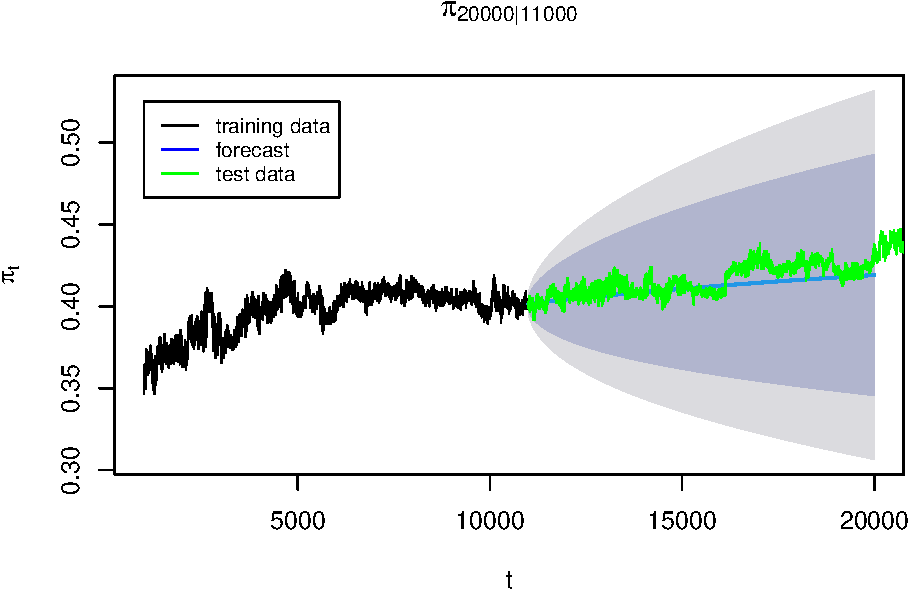
\includegraphics{paper_files/figure-latex/unnamed-chunk-20-1.pdf}
\caption{Forecasts from regression with ARIMA errors model.}
\label{fig:theory}
\end{figure}

The forecasts extend much further into the future and follow the gradual
upward trend more faithfully than the pure ARIMA model.

For comparison, we also fit an ARIMA$(1,1,2)$ model with drift:

\begin{verbatim}
##           ar1           ma1           ma2         drift
##  8.472755e-01 -1.396547e+00  4.324823e-01  4.695287e-06
\end{verbatim}

The drift coefficient is small but positive. Over long horizons, this
accumulates to produce an upward trend (Figure~\ref{fig:drift}).

\begin{figure}
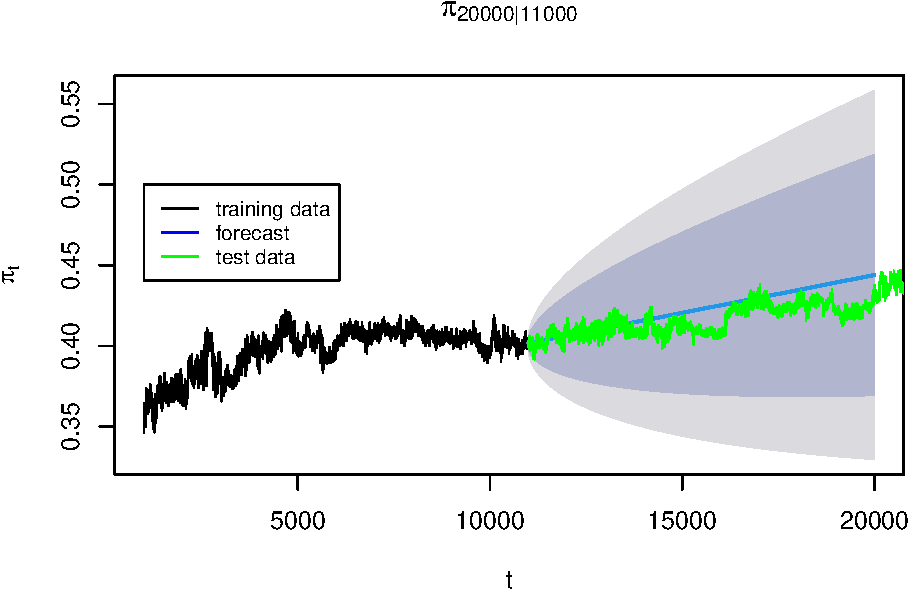
\includegraphics{paper_files/figure-latex/unnamed-chunk-22-1.pdf}
\caption{Forecasts from ARIMA$(1,1,2)$ with drift.}
\label{fig:drift}
\end{figure}

However, ARIMA with drift implies linear growth, which is theoretically
inappropriate: $\pi_t$ must remain bounded in $[0,1]$. The logarithmic
regression model better respects this constraint.

\hypertarget{future-work-dynamic-regression-on-co-variates}{%
\section{Future work: incorporating
covariates}\label{future-work-dynamic-regression-on-co-variates}}

\label{sec:future} Our forecasting models use only lagged values of
$\pi_t$ to predict future confidentiality. This approach captures temporal
patterns but ignores potential covariates that may affect adversary
performance. Incorporating such covariates could improve forecast accuracy
and provide insights into factors driving confidentiality degradation.

\subsection{Information-theoretic covariates}

The adversary learns from observing ciphers $\{c_t\}$, but not all
observations are equally informative. We could model the information
content of each observation explicitly.

Define the information content of observation $t$ as
\begin{equation}
  I_t = -\log_2 \Pr(\operatorname{g}(c_t))\,,
\end{equation}
measured in bits. Observations with low probability under the adversary's
model carry more information.

Lagged values of $I_t$ could be used as predictors in a dynamic regression:
\begin{equation}
  \Pi_t = \beta_0 + \beta_1 I_{t-1} + \beta_2 I_{t-2} + \cdots + \eta_t\,.
\end{equation}
Alternatively, cumulative information (empirical entropy) could serve as
a covariate. This would allow the model to adapt to the informativeness
of recent queries, potentially tightening prediction intervals during
periods of rapid learning.

\subsection{Side-channel information}

Beyond the cipher sequence, the adversary may obtain side-channel
information. For example:
\begin{itemize}
\item Timing information revealing query complexity
\item Access patterns indicating document relevance
\item External knowledge narrowing the plaintext space
\end{itemize}

Such events could be modeled as intervention variables or structural
breaks. For instance, if the adversary learns that cipher $c'$ maps to
a subset $\set{W} \subset \set{X}$, this constitutes an information gain
equivalent to reducing the entropy of the plaintext distribution. Dynamic
regression could incorporate indicator variables for such events, allowing
the model to capture sudden jumps in adversary accuracy.

\hypertarget{conclusion}{%
\section{Conclusion}\label{conclusion}}

We have developed time series models to forecast confidentiality
degradation in encrypted search systems under known-plaintext attacks.
Our analysis demonstrates that standard ARIMA models can capture the
temporal dynamics of adversary accuracy, while dynamic regression with
logarithmic trend terms better incorporates domain knowledge about the
theoretical behavior of learning curves.

\subsection{Model comparison}

The pure ARIMA$(1,1,2)$ model provides reasonable short-term forecasts
and has the virtue of simplicity. However, it lacks theoretical grounding:
ARIMA with drift predicts unbounded growth, eventually yielding
impossible values ($\pi_t > 1$).

The logarithmic regression model ($\pi_t = \beta_0 + \beta_1 \log t +
\eta_t$) better reflects the expected learning dynamics. While it also
lacks an asymptote (eventually predicting $\pi_t > 1$ after approximately
$1.5 \times 10^{15}$ observations), this occurs far beyond any practical
time horizon. The logarithmic form approximates the saturation behavior
of adversary learning reasonably well over finite horizons.

\subsection{Security policy implications}

Consider a security threshold $\pi^* = 0.44$. Using our models, we
estimate the critical time $T^*$ at which confidentiality falls below
this threshold. Figure~\ref{fig:tstar} shows $\hat{T}^*$ as a function
of $\pi^*$.

\begin{figure}
    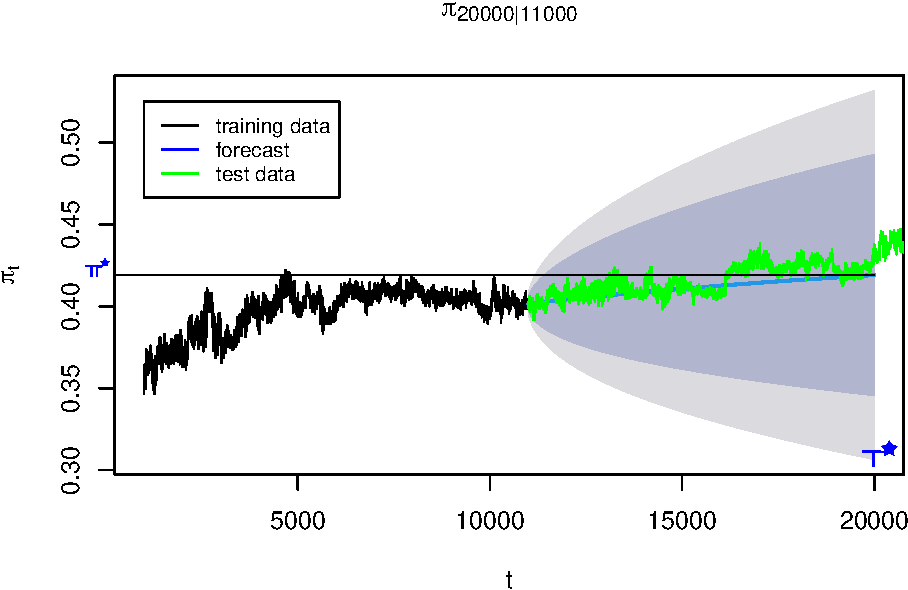
\includegraphics{Tstar.pdf}
    \caption{Estimated critical time $\hat{T}^*$ versus security threshold $\pi^*$.}
    \label{fig:tstar}
\end{figure}

For $\pi^* = 0.44$, we estimate $\hat{T}^* \approx 20000$, suggesting
password reset should occur before 20,000 queries to maintain the
threshold.

However, the 80\% prediction intervals are substantially more conservative,
sometimes recommending near-immediate password reset. This conservatism
limits practical utility: overly frequent resets impose costs on users
and administrators.

\subsection{Limitations and future directions}

The wide prediction intervals indicate substantial forecast uncertainty.
This may stem from model misspecification or from genuine stochasticity
in the adversary's learning process. As discussed in Section~\ref{sec:future},
incorporating covariates (information content of queries, side-channel
events) could reduce uncertainty and improve forecast accuracy.

Alternative model formulations (Gompertz curves, logistic growth models)
that explicitly impose asymptotic bounds merit investigation. Such models
would better respect the theoretical constraint $\pi_t \in [0,1]$ and
might yield more realistic long-term forecasts.

Despite these limitations, our analysis demonstrates that time series
methods can provide quantitative guidance for encrypted search security
policies, enabling data-driven decisions about system reinitialization
timing.



\bibliography{refs.bib}
\bibliographystyle{plainurl}

\end{document}
